\documentclass{beamer}
\usetheme{Madrid}
\usecolortheme{beaver}
\usepackage[utf8]{inputenc}
\usefonttheme{professionalfonts}
\usepackage[ngerman]{babel}
\usepackage{tikz}
\usetikzlibrary{arrows,shapes,positioning}
\usepackage{pifont}
\newcommand{\cmark}{\ding{51}}%
\newcommand{\qmark}{\ding{51} / \ding{55}}%
\newcommand{\xmark}{\ding{55}}%
\newcommand{\COO}{$\mathrm{CO}_2$}%
\newcommand{\imply}{$\Rightarrow$}
\title[Kipppunkte]{
  Visualisierung der Hysterese\\
  von Kipppunkten}
\subtitle{Impulsvortrag mit anschließender Diskussion}
\author{Jürgen Reuter}
\institute[\tt{soundpaint.org}]{\tt{soundpaint.org}}
\date[LFF2023]{Letters for Future, 30. September 2023}

\AtBeginSection[] {
  \begin{frame}
    \frametitle{Überblick}
    \tableofcontents[currentsection]
  \end{frame}
}

\begin{document}

\tikzstyle{every picture}+=[remember picture]
\everymath{\displaystyle}

\frame{\titlepage}

%\begin{frame}
%  \frametitle{Überblick}
%  \tableofcontents
%\end{frame}

% \section{Kipp{\em punkt} vs. Kipp{\em bereich}}

\begin{frame}
  \frametitle{Kipp{\em punkt}?}
  \tikz[remember picture, overlay] {
    \node[shift={(0.45cm, 0.50cm)}] at (current page.south west) (t1) {
      \begin{tikzpicture}[remember picture, overlay]
        \draw<2->[step=0.5cm,gray!30!white,very thin] (0.1, 0.1) grid (10.4, 3.9);
      \end{tikzpicture}
    }
  }
  \tikz[remember picture, overlay] {
    \node[shift={(0.50cm, 0.50cm)}] at (current page.south west) (t2) {
      \begin{tikzpicture}[remember picture, overlay]
        {\color<2>{blue}
          \draw<2->[thick,->](0.0, 0.5) -- (10.5, 0.5) node[anchor=north west] {\scriptsize \COO};
        }
      \end{tikzpicture}
    }
  }
  \tikz[remember picture, overlay] {
    \node[shift={(0.50cm, 0.50cm)}] at (current page.south west) (t3) {
      {\color<3>{blue}
        \begin{tikzpicture}[remember picture, overlay]
          \draw<3->[thick,->](0.5, 0.0) -- (0.5, 4.0) node[anchor=south west] {\scriptsize Effekt};
        \end{tikzpicture}
      }
    }
  }
  \tikz[remember picture, overlay] {
    \node[shift={(0.50cm, 0.50cm)}] at (current page.south west) (t4) {
      {\color<4>{blue}
        \begin{tikzpicture}[remember picture, overlay]
          \draw<4->(1.0, 1.0) -- (5.5, 1.0);
        \end{tikzpicture}
      }
    }
  }
  \tikz[remember picture, overlay] {
    \node[shift={(0.50cm, 0.50cm)}] at (current page.south west) (t5) {
      {\color<5>{blue}
        \begin{tikzpicture}[remember picture, overlay]
          \draw<5->(5.5, 3.5) -- (10.0, 3.5);
        \end{tikzpicture}
      }
    }
  }
  \tikz[remember picture, overlay] {
    \node[shift={(0.50cm, 0.50cm)}] at (current page.south west) (t6) {
      {\color<6>{blue}
        \begin{tikzpicture}[remember picture, overlay]
          \draw<6->[dashed](5.5, 1.0) -- (5.5, 3.5);
        \end{tikzpicture}
      }
    }
  }
  \vspace{-3.5cm}\\
  Naive Vorstellung: Punktförmige Schwelle
  \begin{itemize}
    \item<2-> \color<2>{blue} Reellwertige Größe (z.B. \COO-Gehalt der Luft)
    \item<3-> \color<3>{blue} bewirkter Zustand (\glqq{}Effekt\grqq)
    \item<4-> \color<4>{blue} Zustand 1 (\glqq{}jetziges Klima\grqq)
    \item<5-> \color<5>{blue} Zustand 2 (\glqq{}zukünftiges Klima\grqq)
    \item<6-> \color<6>{blue} Abrupter Wechsel (\glqq{}Kipppunkt\grqq)
  \end{itemize}
\end{frame}

\begin{frame}
  \frametitle{Kipp{\em bereich}!}
  \tikz[remember picture, overlay] {
    \node[shift={(0.45cm, 0.50cm)}] at (current page.south west) (t1) {
      \begin{tikzpicture}[remember picture, overlay]
        \draw<1->[step=0.5cm,gray!30!white,very thin] (0.1, 0.1) grid (10.4, 3.9);
      \end{tikzpicture}
    }
  }
  \tikz[remember picture, overlay] {
    \node[shift={(0.50cm, 0.50cm)}] at (current page.south west) (t2) {
      \begin{tikzpicture}[remember picture, overlay]
        \draw<1->[thick,->](0.0, 0.5) -- (10.5, 0.5)
        node[anchor=north west] {\scriptsize \COO};
      \end{tikzpicture}
    }
  }
  \tikz[remember picture, overlay] {
    \node[shift={(0.45cm, 0.50cm)}] at (current page.south west) (t3) {
      \begin{tikzpicture}[remember picture, overlay]
        \draw<1->[thick,->](0.5, 0.0) -- (0.5, 4.0)
        node[anchor=south west] {\scriptsize Effekt};
      \end{tikzpicture}
    }
  }
  \tikz[remember picture, overlay] {
    \node[shift={(0.50cm, 0.50cm)}] at (current page.south west) (t4) {
      {\color<2>{blue}
        \begin{tikzpicture}[remember picture, overlay]
          \draw<2->(1.0, 1.0) -- (6.0, 1.0)
          node[anchor=north]{Zustand 1};
        \end{tikzpicture}
      }
    }
  }
  \tikz[remember picture, overlay] {
    \node[shift={(0.50cm, 0.50cm)}] at (current page.south west) (t5) {
      {\color<3>{blue}
        \begin{tikzpicture}[remember picture, overlay]
          \draw<3->(5.0, 3.5) -- (10.0, 3.5)
          node[anchor=south]{Zustand 2};
        \end{tikzpicture}
      }
    }
  }
  \tikz[remember picture, overlay] {
    \node[shift={(0.50cm, 0.50cm)}] at (current page.south west) (t6) {
      {\color<4>{blue}
        \begin{tikzpicture}[remember picture, overlay]
          \draw<4->[thick,->] (6.0, 1.0) -- (7.5, 3.5);
        \end{tikzpicture}
      }
    }
  }
  \tikz[remember picture, overlay] {
    \node[shift={(0.50cm, 0.50cm)}] at (current page.south west) (t7) {
      {\color<5>{blue}
        \begin{tikzpicture}[remember picture, overlay]
          \draw<5->[thick,<-](3.5, 1.0) -- (5.0, 3.5);
        \end{tikzpicture}
      }
    }
  }
  \tikz[remember picture, overlay] {
    \node[shift={(0.50cm, 0.50cm)}] at (current page.south west) (t8) {
      {\color<6>{blue}
        \begin{tikzpicture}[remember picture, overlay]
          \draw<6->[thick,<->](4.25, 2.25) -- (6.75, 2.25)
          node[anchor=south east]{Hysterese};
        \end{tikzpicture}
      }
    }
  }
  \vspace{-3.5cm}\\
  Hysterese
  \begin{itemize}
    \item<2-> \color<2>{blue} Zustand 1 (\glqq{}jetziges Klima\grqq)
    \item<3-> \color<3>{blue} Zustand 2 (\glqq{}zukünftiges Klima\grqq)
    \item<4-> \color<4>{blue} Wechselbereich Zustand 1 {\imply} 2
    \item<5-> \color<5>{blue} Wechselbereich Zustand 2 {\imply} 3
    \item<6-> \color<6>{blue} \glqq{}Hysterese\grqq
  \end{itemize}
\end{frame}

\begin{frame}
  \frametitle{Alternative Hystereseformen}
  \begin{itemize}
    \item<1-> \color<1>{blue} Bisher: Form eines Parallelogramm
    \item<2-> \color<2>{blue} Realität: Keine Ecken
    \item<3-> \color<3>{blue} Sondern kurvige Form
    \item<4-> \color<4>{blue} Schleifenartige Form
  \end{itemize}
\end{frame}

\begin{frame}
  \frametitle{Beispiele aus Physik, Technik und Natur, Wirtschaft}
  Hysterese-Effekte gibt es sehr häufig:
  \begin{itemize}
    \item<2-> \color<2>{blue} Wippe
    \item<3-> \color<3>{blue} Prellfreier Schwellwertschalter (Schmitt-Trigger)
    \item<4-> \color<4>{blue} Bistabile Kippschaltungen (z.B. Flipflop)
    \item<5-> \color<5>{blue} Ferromagnetische Magnetisierung
    \item<5-> \color<5>{blue} KI / Neuronen: Sigmoid-Aktivierung + Rückkopplung
    \item<6-> \color<6>{blue} Diverse ökonomische / soziale Prozesse
    \item<7-> \color<7>{blue} Schmelze weiß reflektierender Schneeflächen
    \item<8-> \color<8>{blue} Permafrostende: Freiwerdendes gebundenes Methangas
  \end{itemize}
\end{frame}

% \section{Beispiele}

\begin{frame}
  \frametitle{Beispiel Wippe}
  \tikz[remember picture, overlay] {
    \node[shift={(0.50cm, 0.50cm)}] at (current page.south west) (t1) {
      \begin{tikzpicture}[remember picture, overlay]
        \node<2-> (seesaw) at (100.0pt, 55.0pt)
                  {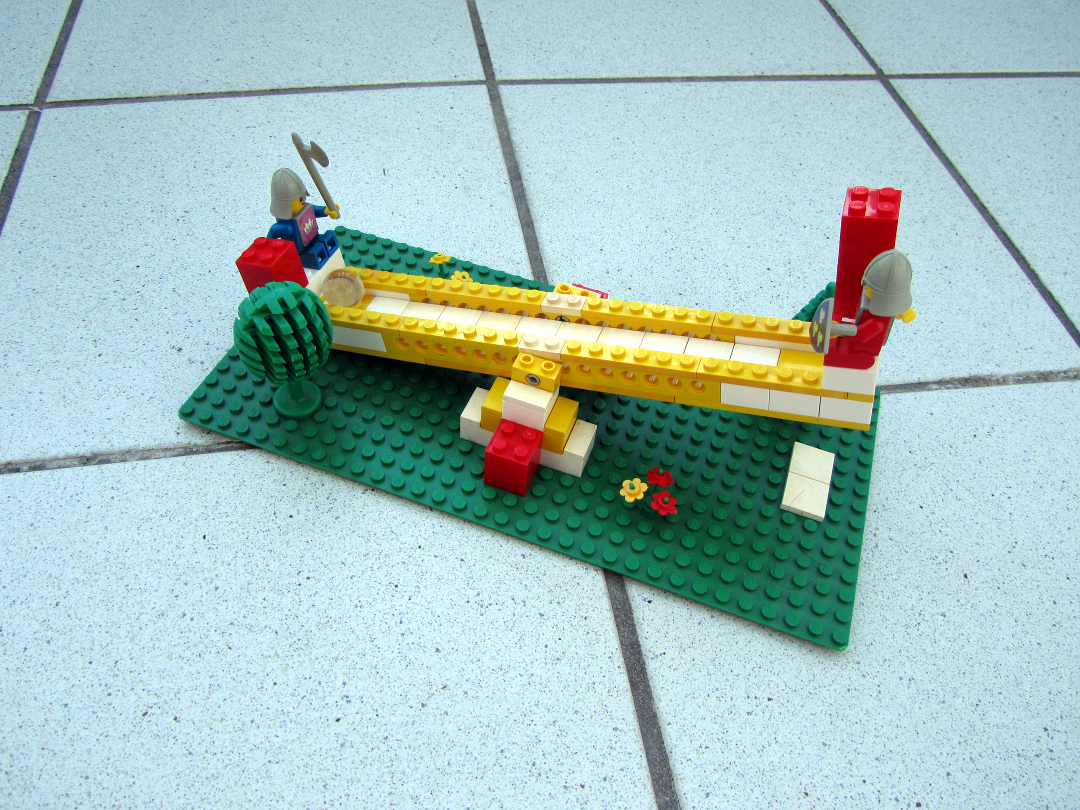
\includegraphics[width=200pt]{../images/seesaw.png}};
      \end{tikzpicture}
    }
  }
  \tikz[remember picture, overlay] {
    \node[shift={(0.50cm, 0.50cm)}] at (current page.south west) (t1) {
      {\color<3->{red}
        \begin{tikzpicture}[remember picture, overlay]
          \draw<3->[->,very thick](85.0pt, 135.0pt) -- (65.0pt, 75.0pt);
        \end{tikzpicture}
      }
    }
  }
  \vspace{-3.5cm}\\
  Präparierung mit Kugel
  \begin{itemize}
    \item<2-> \color<2>{blue} Gewöhnliche Wippe: Hysterese vernachlässigbar
    \item<3-> \color<3>{blue} Präparierte Wippe: Rollendes Gewicht im Balken
    \item<4-> \color<4>{blue} Kugel rollt zum unteren Ende
    \item<5-> \color<5>{blue} Hysterese durch Position der Kugel
  \end{itemize}
\end{frame}

\begin{frame}
  \frametitle{Computermodell der Wippe}
  \tikz[remember picture, overlay] {
    \node[shift={(0.50cm, 0.50cm)}] at (current page.south west) (t1) {
      \begin{tikzpicture}[remember picture, overlay]
        \node<2-> (seesaw) at (290.0pt, 145.0pt)
                  {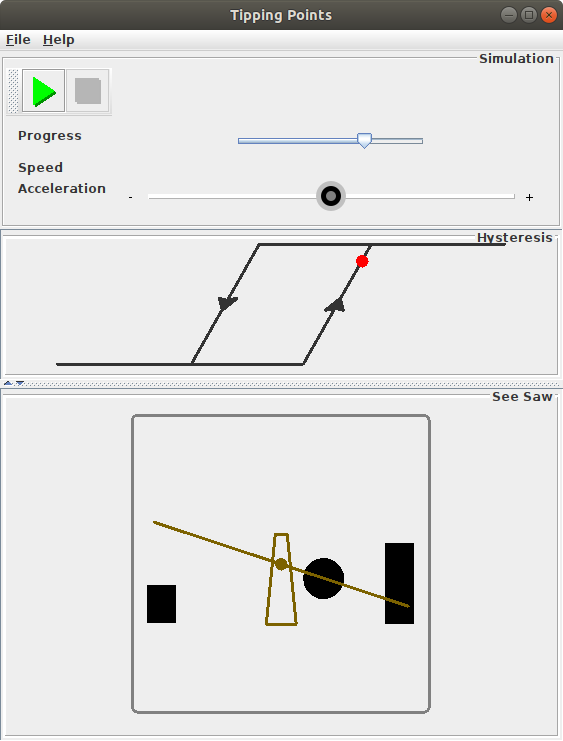
\includegraphics[width=100pt]{../images/screenshot_v0_1.png}};
      \end{tikzpicture}
    }
  }
  \vspace{-2.5cm}\\
  Ein Modell ist ein {\em vereinfachtes} Abbild der Wirklichkeit.
  \begin{itemize}
    \item<2-> \color<2>{blue} Nachbildung Wippe, rollende Kugel
    \item<3-> \color<3>{blue} Vereinfachungen
      \begin{itemize}
        \item<4-> \color<4>{blue} Konstant schnelles Rollen
        \item<5-> \color<5>{blue} Simulationsumkehr vor Wendepunkt\\
          \imply{} Aufwärtsrollen
      \end{itemize}
    \item<6-> \color<6>{blue} Wirklichkeit deutlich komplexer
      \begin{itemize}
        \item<7-> \color<7>{blue} Linear wachsende Geschwindigkeit der Kugel
        \item<8-> \color<8>{blue} Richtungsumkehr: Kugel muss erst Abbremsen
        \item<9-> \color<9>{blue} \imply{} Umkehr zusätzlich erschwert
      \end{itemize}
  \end{itemize}
\end{frame}

\begin{frame}
  \frametitle{\glqq{}Point of No Return\grqq (\glqq{}PNR\grqq)?}
  \tikz[remember picture, overlay] {
    \node[shift={(0.45cm, 0.50cm)}] at (current page.south west) (t1) {
      \begin{tikzpicture}[remember picture, overlay]
        \draw<1->[step=0.5cm,gray!30!white,very thin] (0.1, 0.1) grid (10.4, 3.9);
      \end{tikzpicture}
    }
  }
  \tikz[remember picture, overlay] {
    \node[shift={(0.50cm, 0.50cm)}] at (current page.south west) (t2) {
      \begin{tikzpicture}[remember picture, overlay]
        \draw<1->[thick,->](0.0, 0.5) -- (10.5, 0.5)
        node[anchor=north west] {\scriptsize \COO};
      \end{tikzpicture}
    }
  }
  \tikz[remember picture, overlay] {
    \node[shift={(0.45cm, 0.50cm)}] at (current page.south west) (t3) {
      \begin{tikzpicture}[remember picture, overlay]
        \draw<1->[thick,->](0.5, 0.0) -- (0.5, 4.0)
        node[anchor=south west] {\scriptsize Effekt};
      \end{tikzpicture}
    }
  }
  \tikz[remember picture, overlay] {
    \node[shift={(0.50cm, 0.50cm)}] at (current page.south west) (t4) {
      \begin{tikzpicture}[remember picture, overlay]
        \draw<1->(1.0, 1.0) -- (6.0, 1.0)
        node[anchor=north]{Zustand 1};
      \end{tikzpicture}
    }
  }
  \tikz[remember picture, overlay] {
    \node[shift={(0.50cm, 0.50cm)}] at (current page.south west) (t5) {
      \begin{tikzpicture}[remember picture, overlay]
        \draw<1->(5.0, 3.5) -- (10.0, 3.5)
        node[anchor=south]{Zustand 2};
      \end{tikzpicture}
    }
  }
  \tikz[remember picture, overlay] {
    \node[shift={(0.50cm, 0.50cm)}] at (current page.south west) (t6) {
      \begin{tikzpicture}[remember picture, overlay]
        \draw<1->[thick,->] (6.0, 1.0) -- (7.5, 3.5);
      \end{tikzpicture}
    }
  }
  \tikz[remember picture, overlay] {
    \node[shift={(0.50cm, 0.50cm)}] at (current page.south west) (t7) {
      \begin{tikzpicture}[remember picture, overlay]
        \draw<1->[thick,<-](3.5, 1.0) -- (5.0, 3.5);
      \end{tikzpicture}
    }
  }
  \tikz[remember picture, overlay] {
    \node[shift={(0.50cm, 0.50cm)}] at (current page.south west) (t8) {
      {\color<3>{red}
        \begin{tikzpicture}[remember picture, overlay]
          \draw<3->[thick,dashed] (7.5, 3.5) circle (0.2cm)
          node[anchor=south east]{?};
        \end{tikzpicture}
      }
    }
  }
  \tikz[remember picture, overlay] {
    \node[shift={(0.50cm, 0.50cm)}] at (current page.south west) (t9) {
      {\color<3>{red}
        \begin{tikzpicture}[remember picture, overlay]
          \draw<3->[thick,dashed] (3.5, 1.0) circle (0.2cm)
          node[anchor=south east]{?};
        \end{tikzpicture}
      }
    }
  }
  \tikz[remember picture, overlay] {
    \node[shift={(0.50cm, 0.50cm)}] at (current page.south west) (t10) {
      {\color<5>{red}
        \begin{tikzpicture}[remember picture, overlay]
          \draw<5->[thick,dashed] (6.75, 2.25) circle (0.2cm)
          node[anchor=south east]{?};
        \end{tikzpicture}
      }
    }
  }
  \tikz[remember picture, overlay] {
    \node[shift={(0.50cm, 0.50cm)}] at (current page.south west) (t11) {
      {\color<5>{red}
        \begin{tikzpicture}[remember picture, overlay]
          \draw<5->[thick,dashed] (4.25, 2.25) circle (0.2cm)
          node[anchor=south east]{?};
        \end{tikzpicture}
      }
    }
  }
  \vspace{-3.5cm}\\
  Ab wann geht es realistischerweise nicht mehr zurück?
  \begin{itemize}
    \item<2-> \color<2>{blue} Im Modell
      \begin{itemize}
        \item<3-> \color<3>{blue} Am Zweigpunkt der Hysteresekurve
      \end{itemize}
    \item<4-> \color<4>{blue} In Realität, Beispiel Wippe
      \begin{itemize}
        \item<5-> \color<5>{blue} Deutlich früher
        \item<6-> \color<6>{blue} Zusatzherausforderung beschleunigte Kugel
        \item<7-> \color<7>{blue} Rollrichtung der Kugel umkehren
        \item<8-> \color<8>{blue} Ist-Geschwindigkeit der Kugel einrechnen\\
          \imply{} Gleichgewicht reicht nicht zum Stoppen
      \end{itemize}
  \end{itemize}
\end{frame}

\begin{frame}
  \frametitle{Beispiel Schneeflächen}
  \tikz[remember picture, overlay] {
    \node[shift={(0.50cm, 0.50cm)}] at (current page.south west) (t1) {
      \begin{tikzpicture}[remember picture, overlay]
        \fill<1->(0.5, 0.5) -- (10.5, 0.5) -- (0.5, 3.0) -- (0.5, 0.5);
        node[anchor=north west] {\scriptsize Boden};
      \end{tikzpicture}
    }
  }
  \tikz[remember picture, overlay] {
    \node[shift={(0.50cm, 0.50cm)}] at (current page.south west) (t2) {
      \begin{tikzpicture}[remember picture, overlay]
        \draw<1->(0.5, 0.5) -- (10.5, 0.5) -- (10.5, 2.0) -- (0.5, 2.0) -- (0.5, 0.5);
        node[anchor=north west] {\scriptsize Schnee};
      \end{tikzpicture}
    }
  }
  \tikz[remember picture, overlay] {
    \node[shift={(0.45cm, 0.50cm)}] at (current page.south west) (t3) {
      \begin{tikzpicture}[remember picture, overlay]
        \draw<1->[thick,->](5.0, 2.0) -- (5.0, 3.0);
        \draw<1->[thick,->](6.0, 2.0) -- (6.0, 3.0);
        \draw<1->[thick,->](7.0, 2.0) -- (7.0, 3.0);
        \draw<1->[thick,->](8.0, 2.0) -- (8.0, 3.0);
        \draw<1->[thick,->](9.0, 2.0) -- (9.0, 3.0);
        \draw<1->[thick,->](10.0, 2.0) -- (10.0, 3.0);
      \end{tikzpicture}
    }
  }
  \tikz[remember picture, overlay] {
    \node[shift={(0.45cm, 0.50cm)}] at (current page.south west) (t4) {
      \begin{tikzpicture}[remember picture, overlay]
        \draw<1->[thick,<-,white](1.0, 1.0) -- (1.0, 3.0);
        \draw<1->[thick,<-,white](2.0, 1.0) -- (2.0, 3.0);
        \draw<1->[thick,<-,white](3.0, 1.0) -- (3.0, 3.0);
        \draw<1->[thick,<-,white](4.0, 1.0) -- (4.0, 3.0);
      \end{tikzpicture}
    }
  }
  \vspace{-3.0cm}\\
  \begin{itemize}
    \item<2-> \color<2>{blue} Zustand 1: Schneedecke alles bedeckend
    \item<3-> \color<3>{blue} \imply{} Schnee reflektiert Licht
    \item<4-> \color<4>{blue} \imply{} Geringe Erwärmung
    \item<5-> \color<5>{blue} \imply{} Neuschnee bleibt liegen
    \item<6-> \color<6>{blue} Zustand 2: Schneedecke komplett geschmolzen
    \item<7-> \color<7>{blue} \imply{} Dunkler Boden absorbiert Licht
    \item<8-> \color<8>{blue} \imply{} Starke Erwärmung
    \item<9-> \color<9>{blue} \imply{} Neuschnee schmilzt weg
  \end{itemize}
\end{frame}

\begin{frame}
  \frametitle{Forschungsfragen}
  zur Hysterese
  \begin{itemize}
    \item<2-> \color<2>{blue} Z.B. Schneeflächen: Wie groß ist die Hysterese?
      \begin{itemize}
        \item<3-> \color<3>{blue} Jahre?
        \item<4-> \color<4>{blue} Jahrzehnte?
      \end{itemize}
    \item<5-> \color<5>{blue} Form der Hysterese?
      \begin{itemize}
        \item<6-> \color<6>{blue} Parallelogramm?
        \item<7-> \color<7>{blue} Schleife?
      \end{itemize}
    \item<8-> \color<8>{blue} Wo ist der PNR?
    \item<9-> \color<9>{blue} Gibt es weitere Einflüsse auf den PNR?
      \begin{itemize}
        \item<10-> \color<10>{blue} Beispiel Wippe: beschleunigte Kugel
        \item<11-> \color<11>{blue} Einfluss Luftfeuchtigkeit auf Niederschlag?
      \end{itemize}
    \item<12-> \color<12>{blue} innere Variablen in Hysterese-Modell berücksichtigen
      \begin{itemize}
        \item<13-> \color<13>{blue} z.B. Kugelposition bei der Wippe
        \item<14-> \color<14>{blue} und Kugelgeschwindigkeit
      \end{itemize}
  \end{itemize}
\end{frame}

\begin{frame}
  \begin{center}
    \Huge{Diskussion eröffnet!}
  \end{center}
\end{frame}

% backup slides

\begin{frame}
  \nocite{Reuter20}
  \nocite{Wikipedia20a}
  \frametitle{Literaturverweise}
  \bibliographystyle{acl}
  \bibliography{lff2023}
\end{frame}

\end{document}

%  Local Variables:
%    coding:utf-8
%    mode:LaTeX
%  End:
